\section{Additional Results}
\label{sec:additional_results}

\subsection{Simulated vs. Empirical Data}
\label{subsec:new_cases_fit}

This compares simulated data from our model with empirical data from Germany. We look at
observed infections, fatality rates, the spread of the B117 mutation, vaccinations and
rapid test demands. Where available we do not only look at aggregated statistics but also
analyze the model fit for age groups.\comment[id=J]{summarize the
fit}\comment[id=HM]{Also need to show simulated total infections somewhere. So far only
ever shown for 2021.}


\begin{figure}[ht]
  \centering
  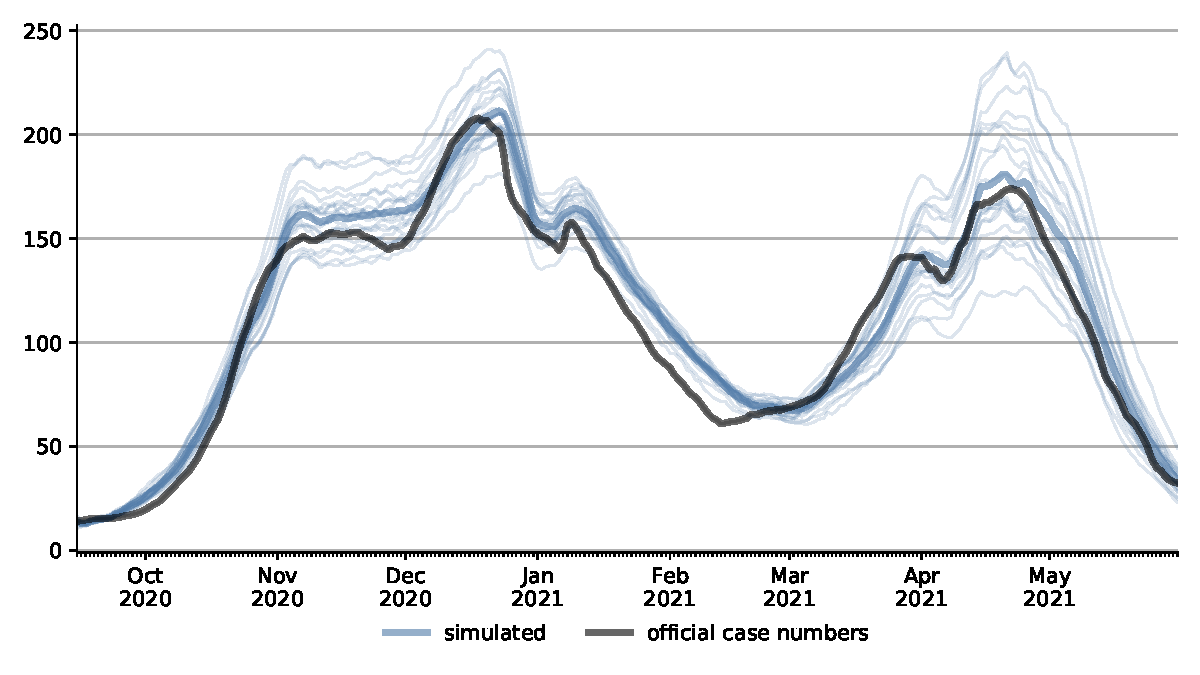
\includegraphics[width=\textwidth]{../figures/results/figures/scenario_comparisons/combined_fit/full_new_known_case_with_single_runs}
  \caption{Simulated and Empirical Infections}
  \figurenotes{The figure shows the weekly incidence rates per 100,000 people for the
  reported versus the simulated infections rates.}
  \label{fig:aggregated_fit2}
\end{figure}


\begin{figure}[ht]
  \centering
  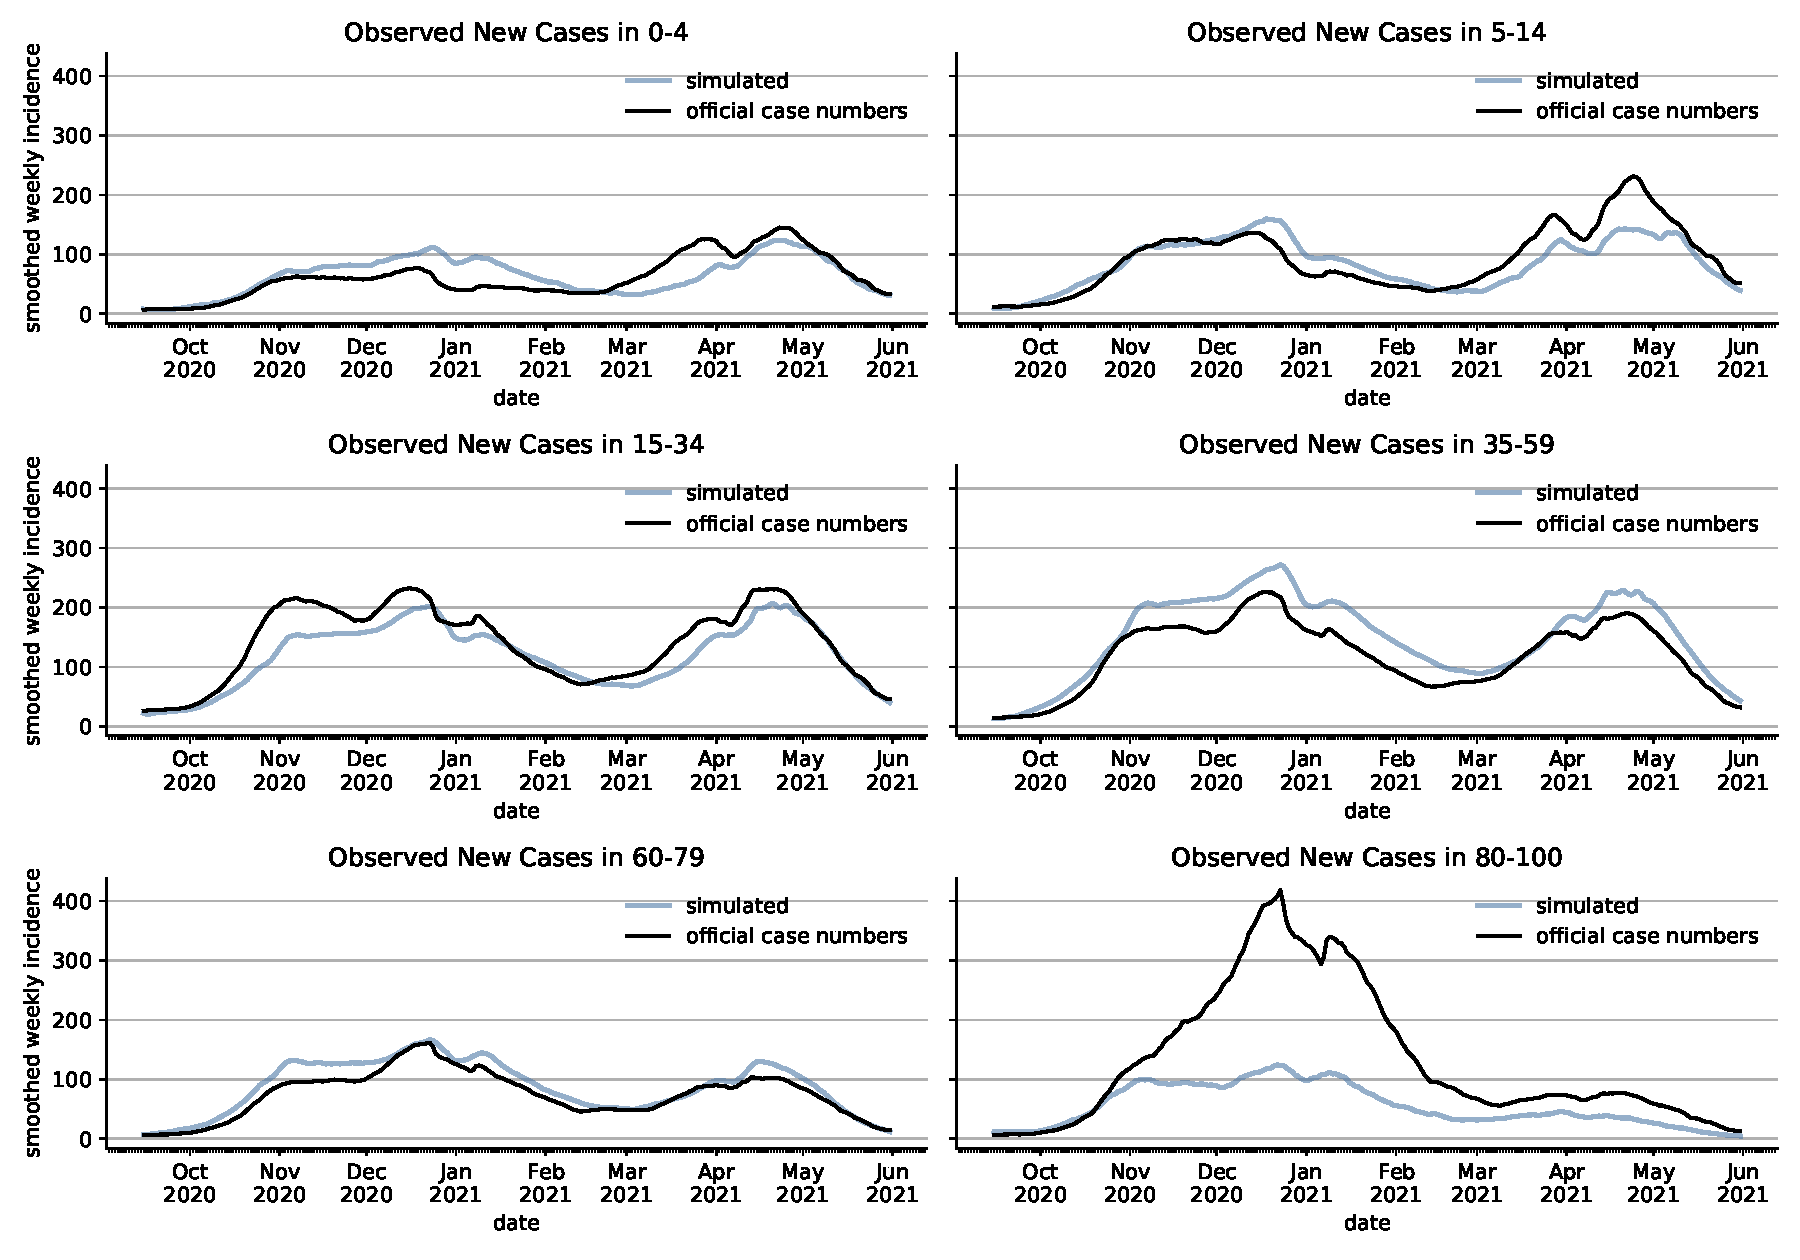
\includegraphics[width=\textwidth]{../figures/results/figures/incidences_by_group/age_group_rki/full_combined_baseline_new_known_case}
  \caption{Simulated and Empirical Infections by Age Group}
  \figurenotes{The figure shows the weekly incidence rates per 100,000 people for the
  reported versus the simulated infections rates for different age groups.}
  \label{fig:age_group_fit}
\end{figure}


\begin{figure}[ht]
  \centering
  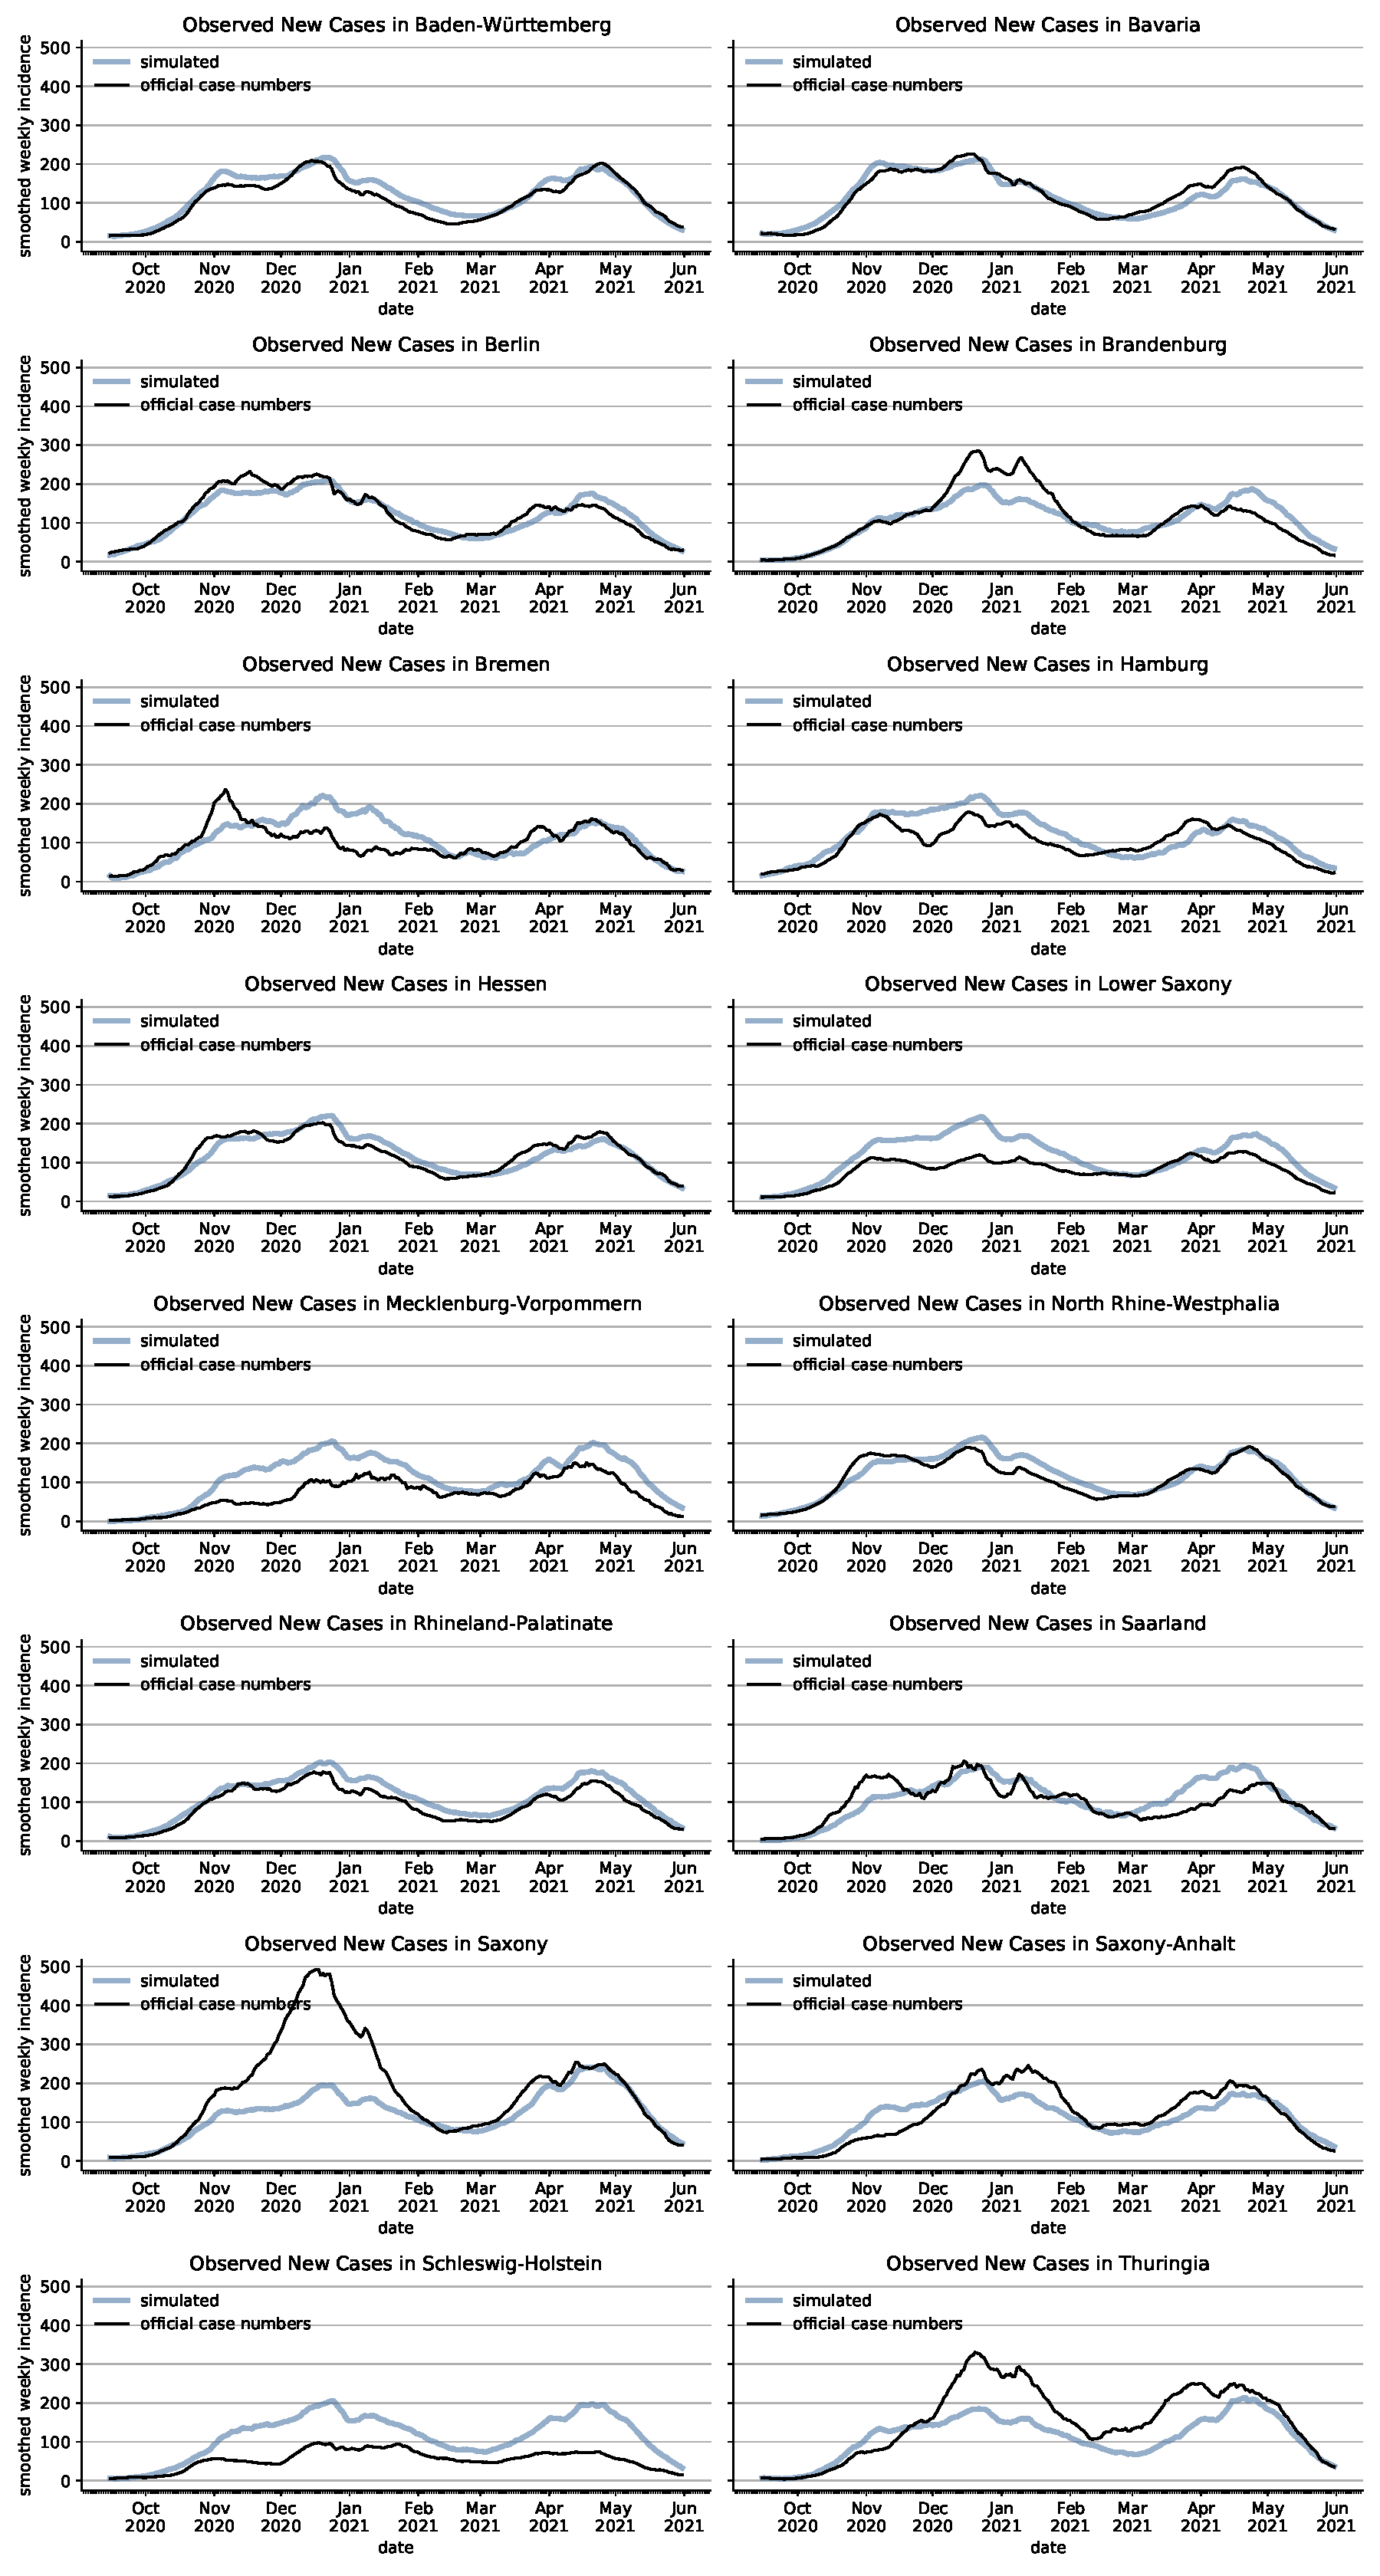
\includegraphics[width=\textwidth]{../figures/results/figures/incidences_by_group/state/full_combined_baseline_new_known_case}
  \caption{Simulated and Empirical Infections by Federal State}
  \figurenotes{The figure shows the weekly incidence rates per 100,000 people for the
  reported versus the simulated infections rates for different federal states.}
  \label{fig:state_fit}
\end{figure}


\FloatBarrier


\subsection{Share of Cases that are Detected  \comment[id=K]{Figure notes missing}}
\label{subsec:appendix_share_known_cases}

\begin{figure}[ht]
  \centering
  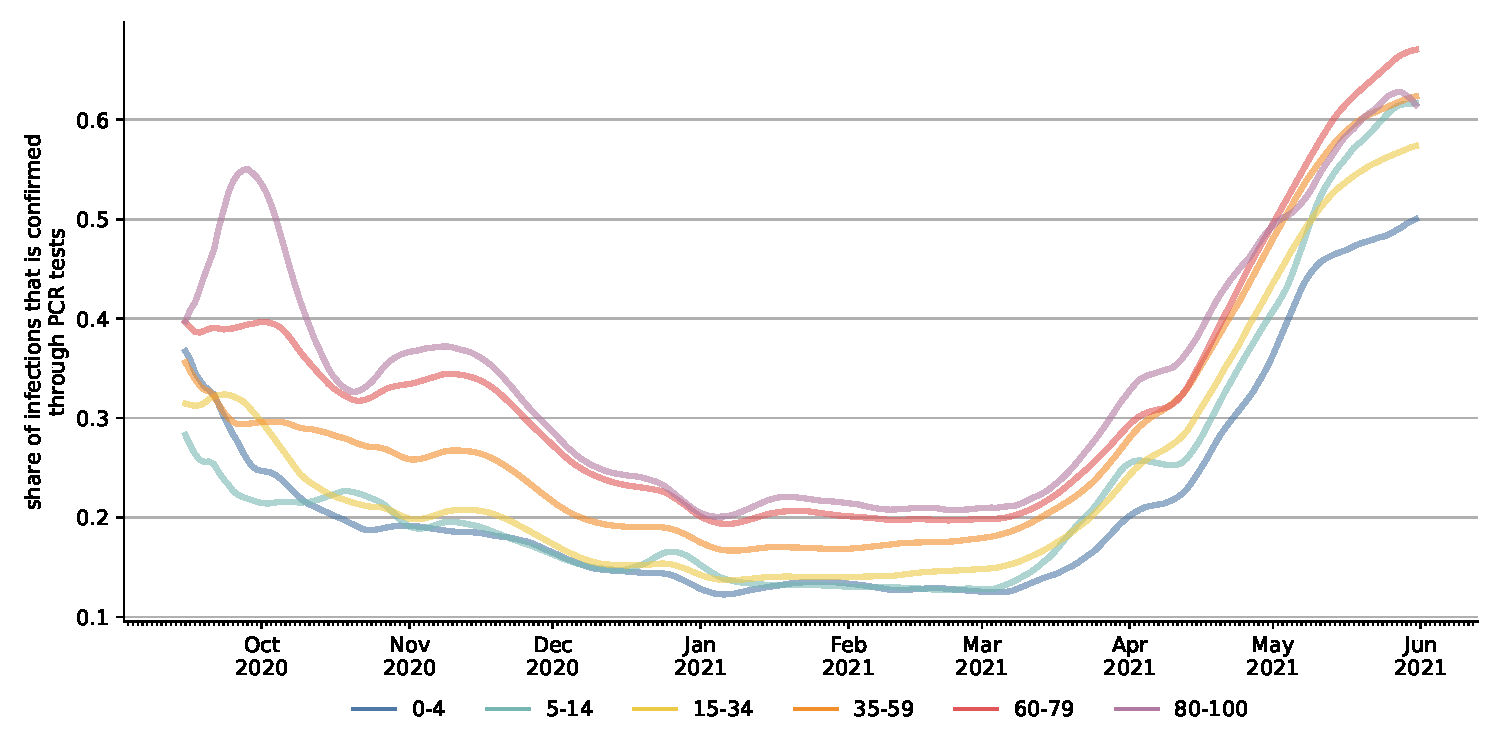
\includegraphics[width=\textwidth]{../figures/results/figures/share_known_cases/full_combined_baseline_by_age_group_rki}
  \caption{Share of Detected Cases by Age Group in the Main Prediction}
  \label{fig:share_known_cases_by_age_group}
  \floatfoot{\noindent}
\end{figure}

It's noteworthy that the share of detected cases increases rapidly in May for the five to
fourteen year olds. This is a direct result of the mandatory tests in
school.

\subsection{Rapid Tests \comment[id=K]{The figures will likely change layout later}}
\label{subsec:appendix_rapid_tests}

\begin{figure}[ht]
  \centering
  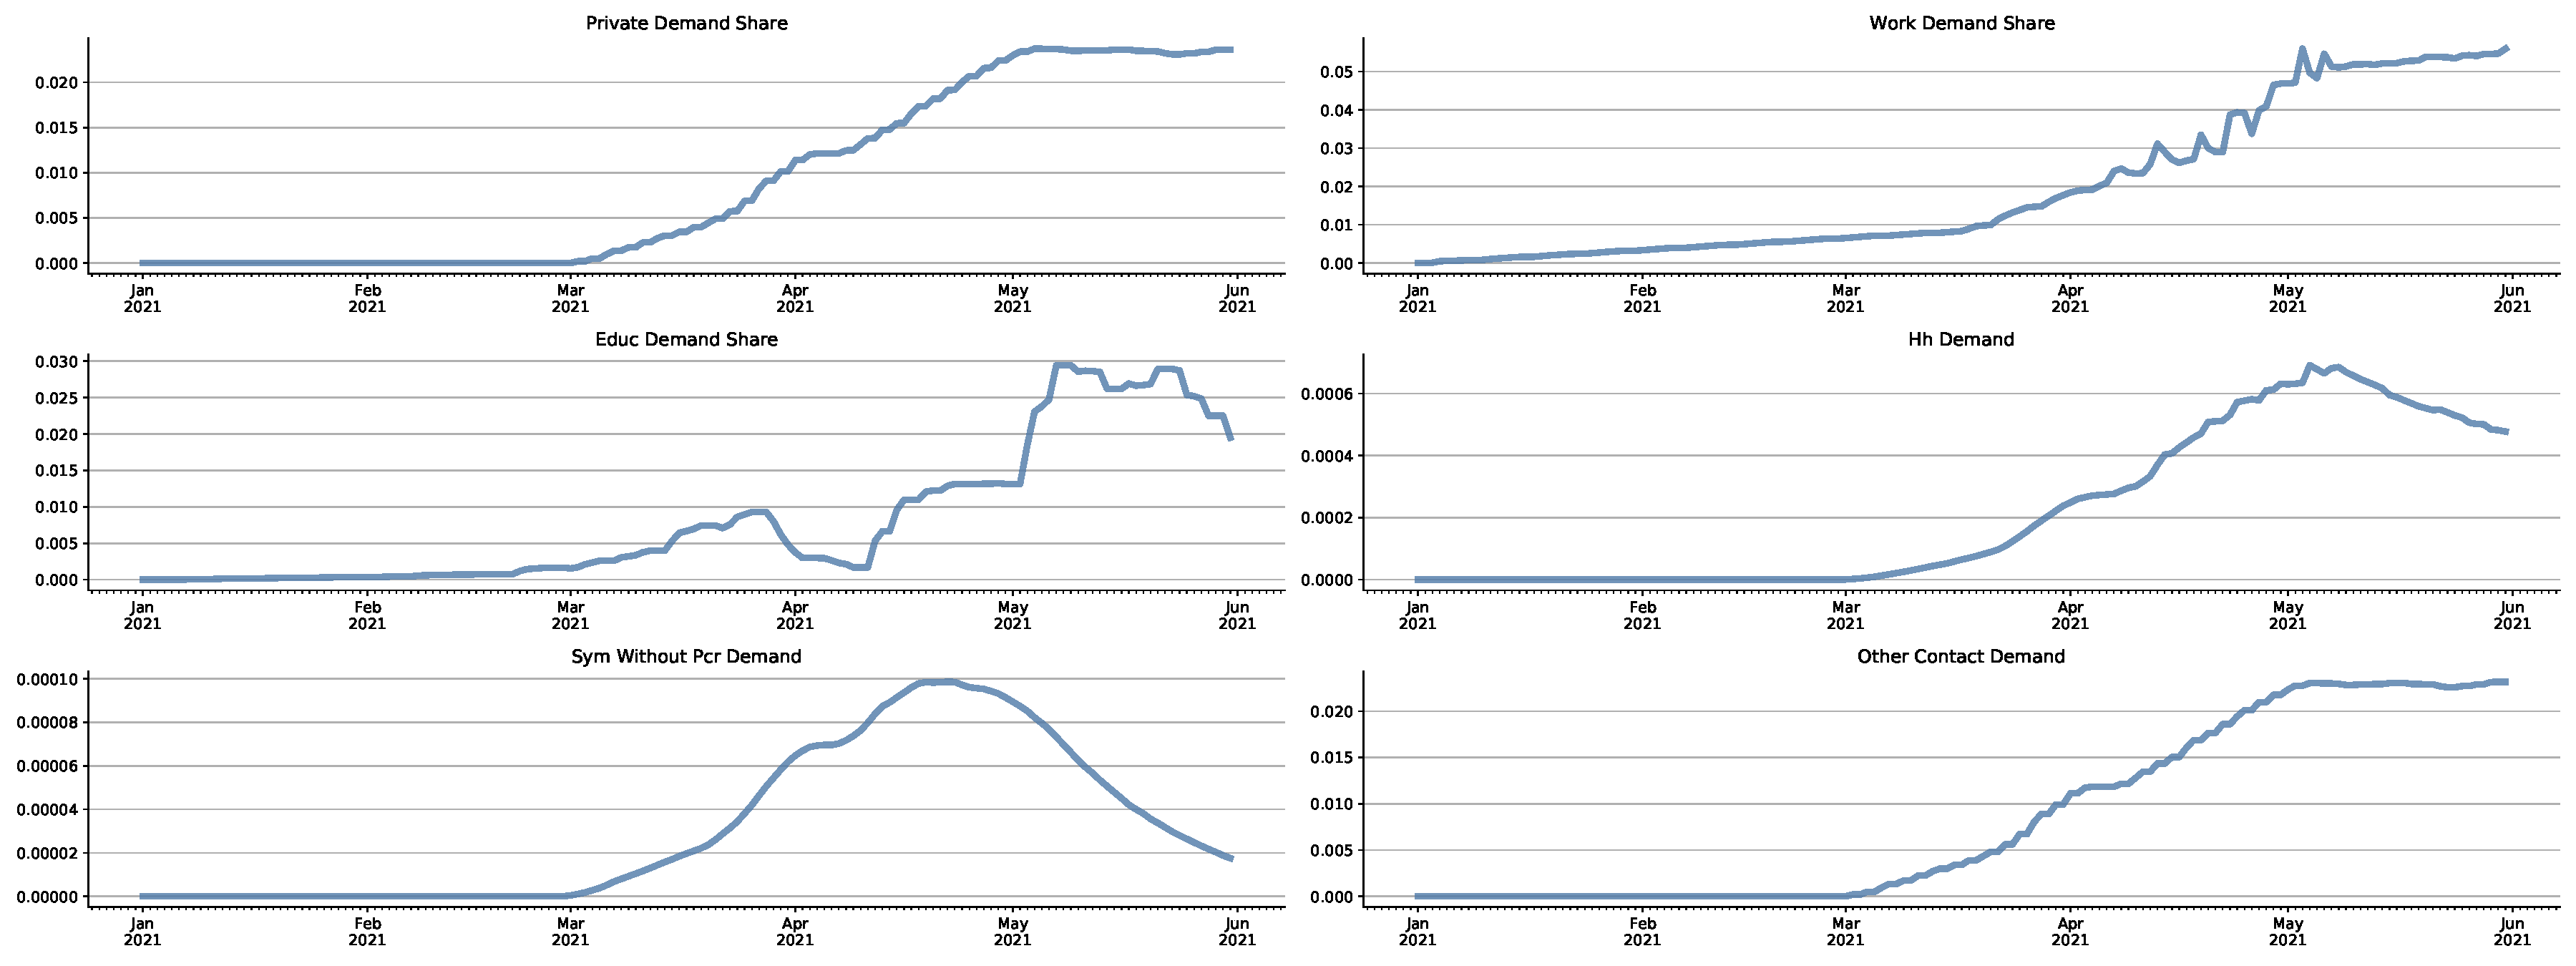
\includegraphics[width=\textwidth]{../figures/results/figures/rapid_test_statistics/demand_shares}
  \caption{Share of the Population Demanding a Rapid Test for a Particular Reason}
  \label{fig:rapid_tests_by_reason}
  \floatfoot{\noindent Note that the lower three (household demand, symptomatic without
  PCR demand and other contact demand together form the private demand category. Also
  note that these do not add up to the total share of demanded rapid tests as individuals
  may have more than one reason to demand a rapid test on any given day. }
\end{figure}

\begin{figure}[ht]
  \centering
  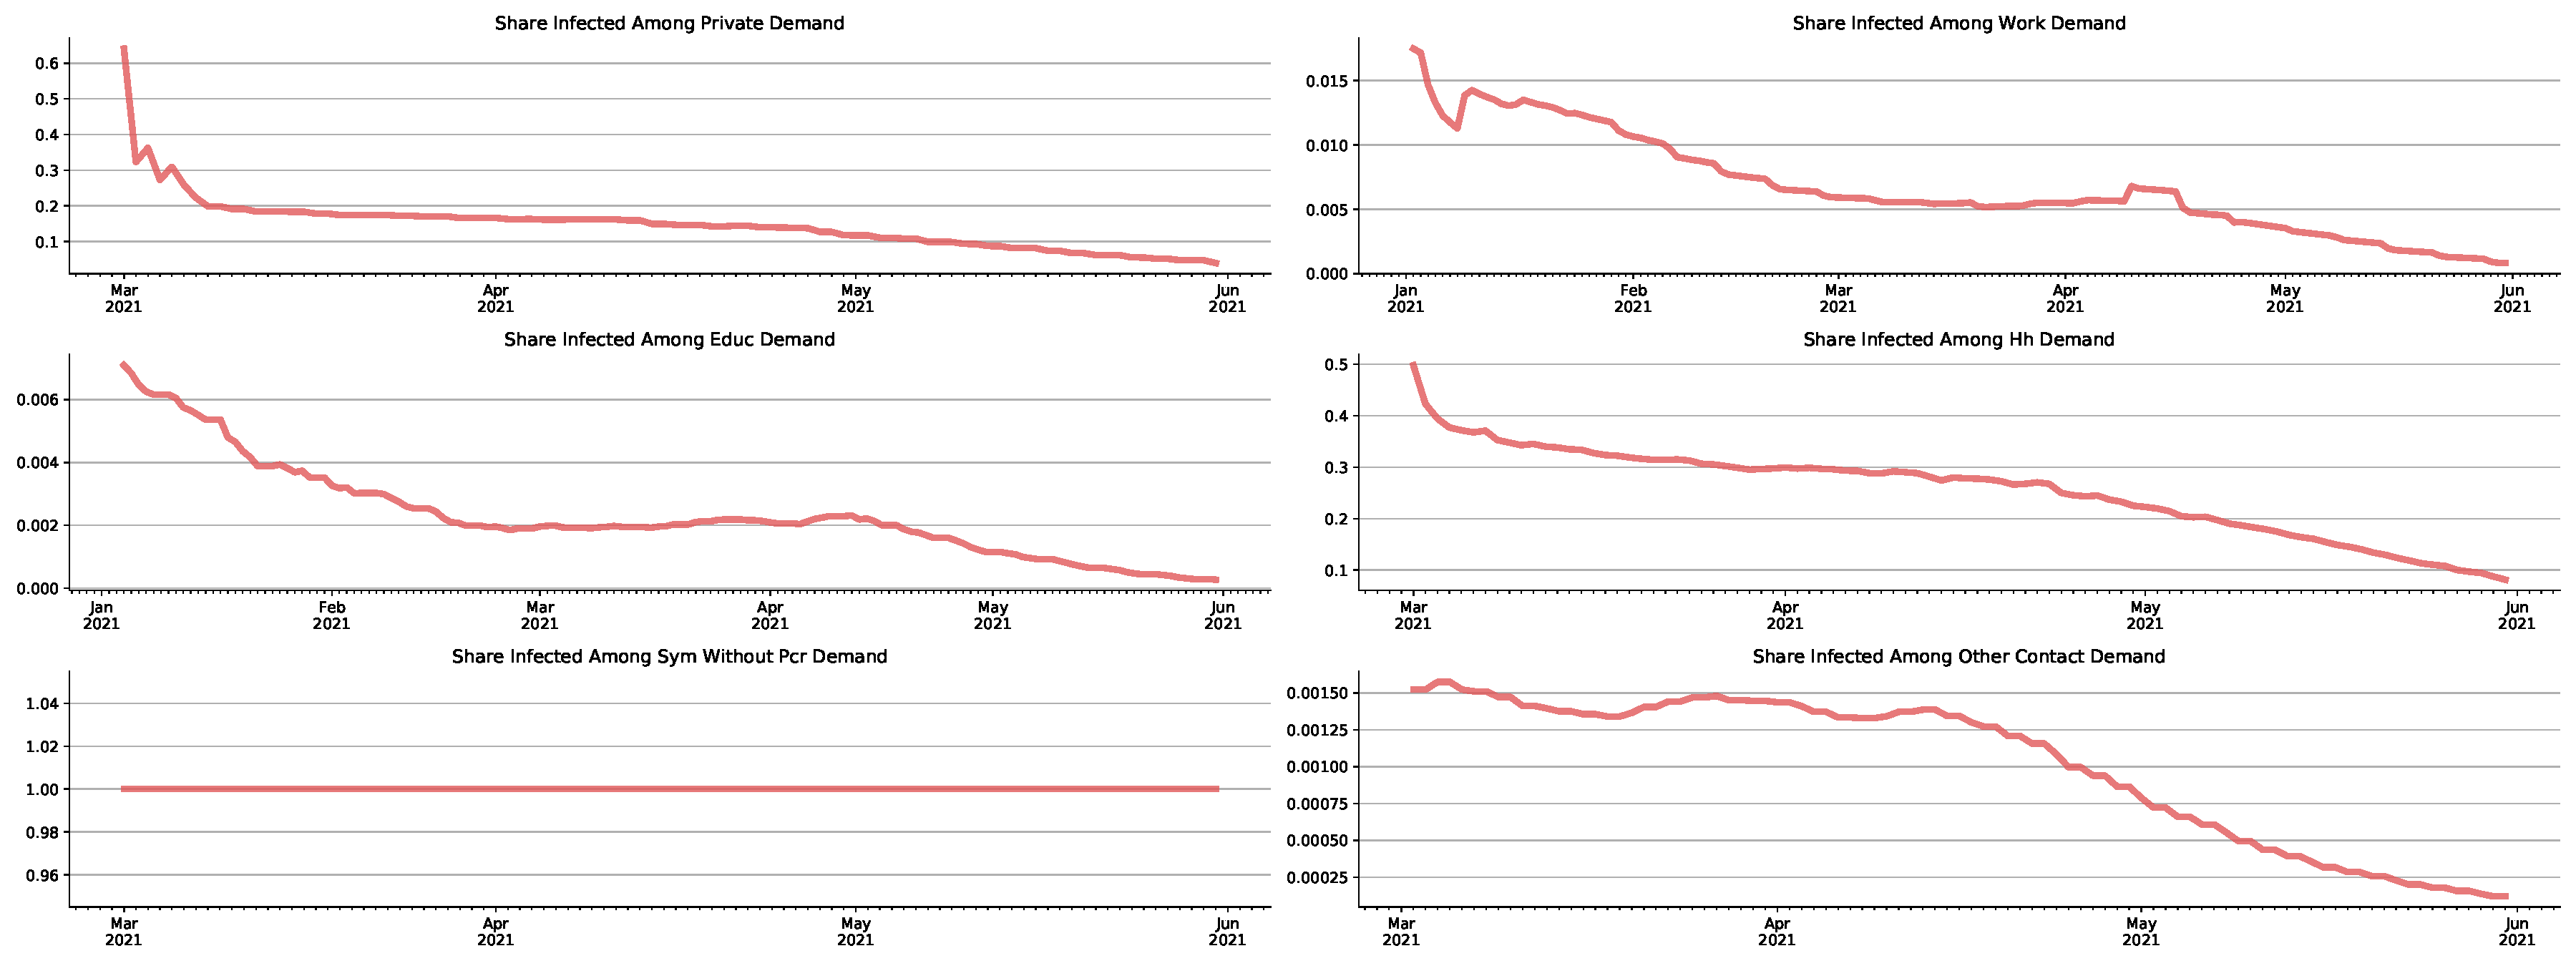
\includegraphics[width=\textwidth]{../figures/results/figures/rapid_test_statistics/share_infected_among_demand}
  \caption{Share of individuals who Demand a Rapid Test for a Particular Reason that are Actually Infected}
  \label{fig:share_of_rapid_tests_by_reason_by_infected}
  \floatfoot{\noindent Note that the lower three (household demand, symptomatic without
  PCR demand and other contact demand together form the private demand category. Also
  note that this is not the same as individuals getting a positive rapid test. The
  sensitivity is quite low before individuals become infectious. Therefore, if
  individuals are still in the latent period of their infection they are likely to get a
  false positive rapid test.}
\end{figure}

\FloatBarrier


\subsection{Scenarios}
\label{subsec:appendix_scenarios}

This is the results section.\comment[id=K]{The results can be found in `figures/results`.
This includes both figures and tables for lookup of numbers and summary tables.}


\begin{figure}[ht]
  \centering
  \begin{subfigure}{.6\textwidth}
    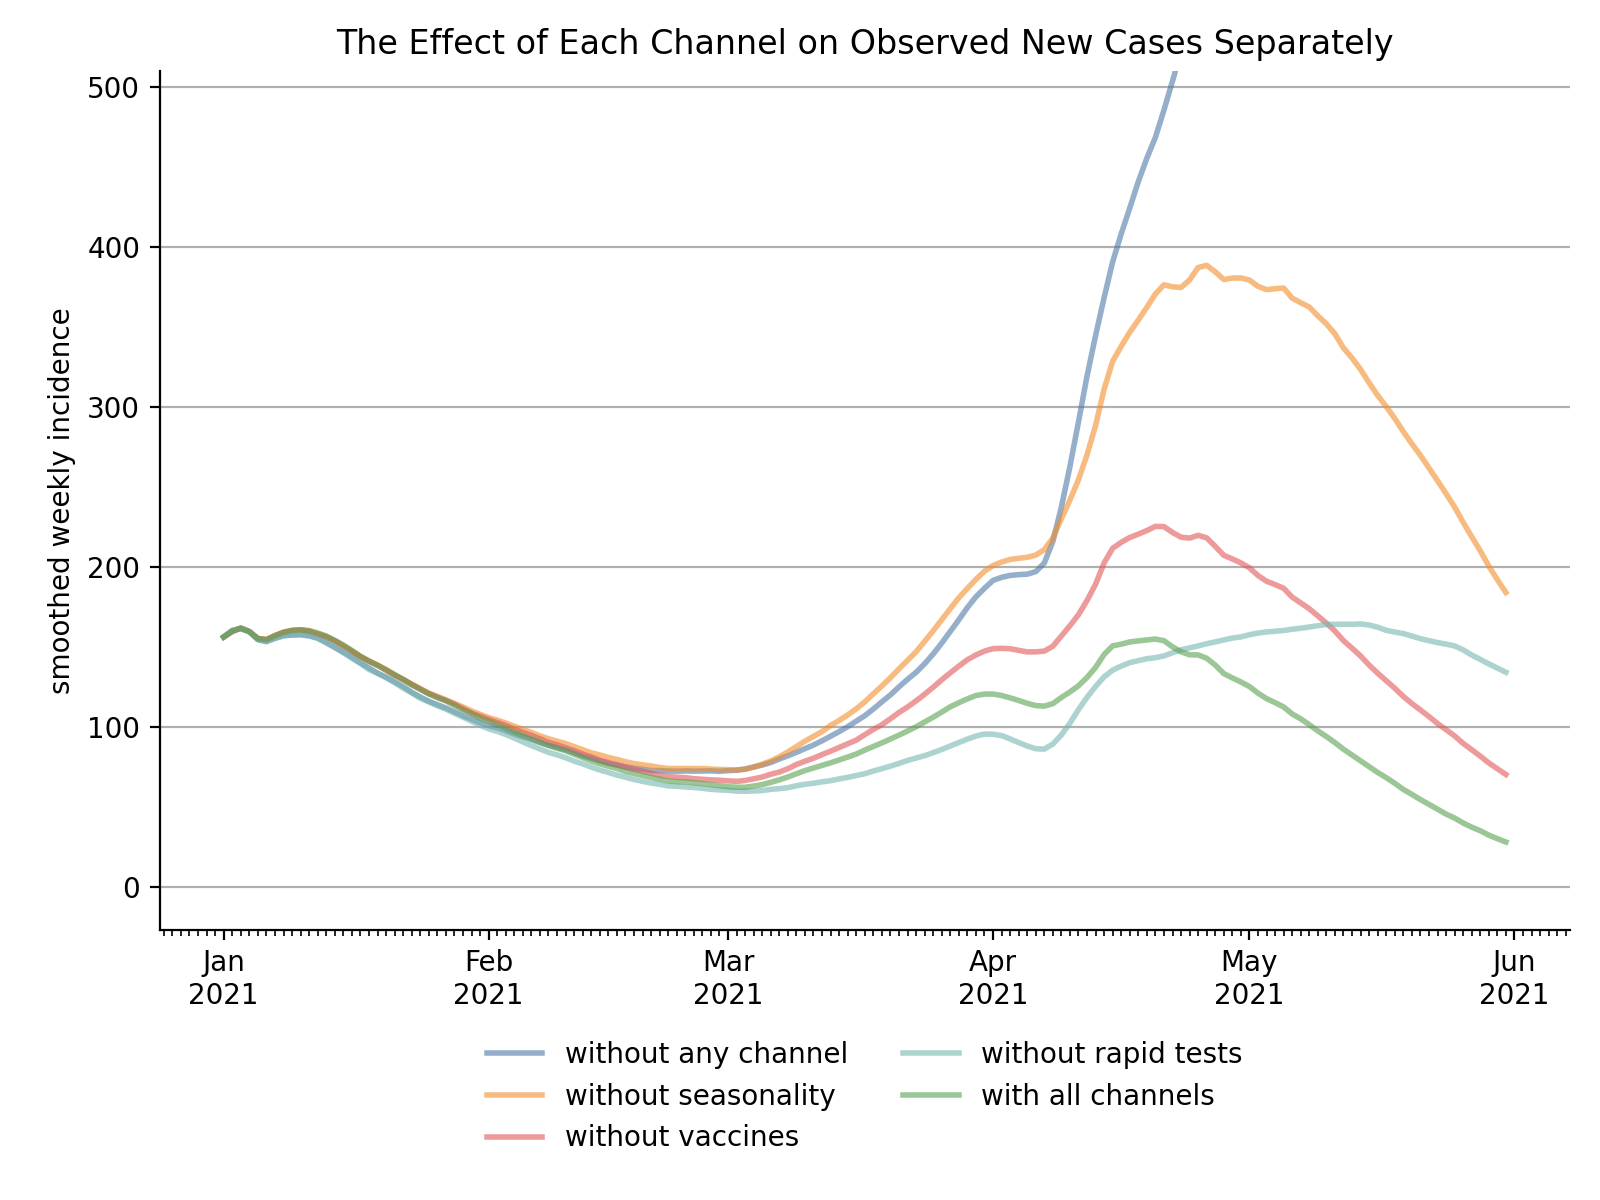
\includegraphics[width=0.9 \textwidth]{../figures/results/figures/scenario_comparisons/one_off_and_combined/full_new_known_case_cropped}
  \end{subfigure}%
  \begin{subfigure}{.6\textwidth}
    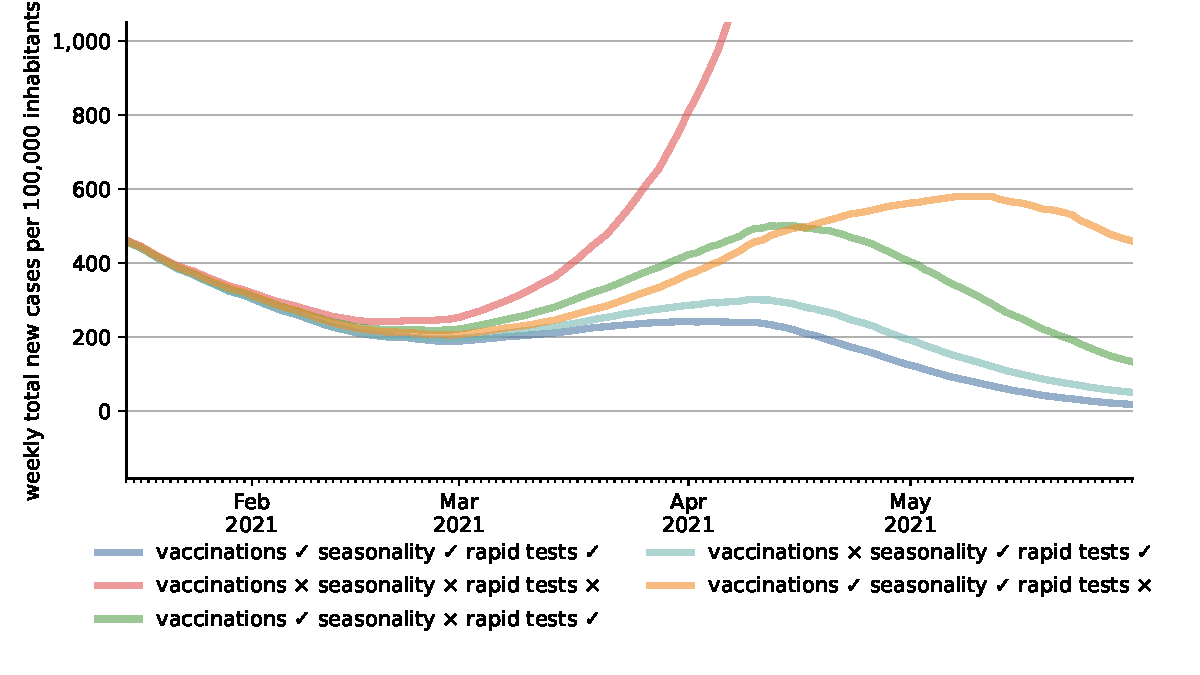
\includegraphics[width=0.9 \textwidth]{../figures/results/figures/scenario_comparisons/one_off_and_combined/full_newly_infected_cropped}
  \end{subfigure}
  \caption{The Effect of Policies on Observed and Unobserved Cases}
  \label{fig:explain_decline}
  \figurenotes{\ldots}
\end{figure}



\begin{figure}[ht]
  \centering
  \begin{subfigure}{.6\textwidth}
    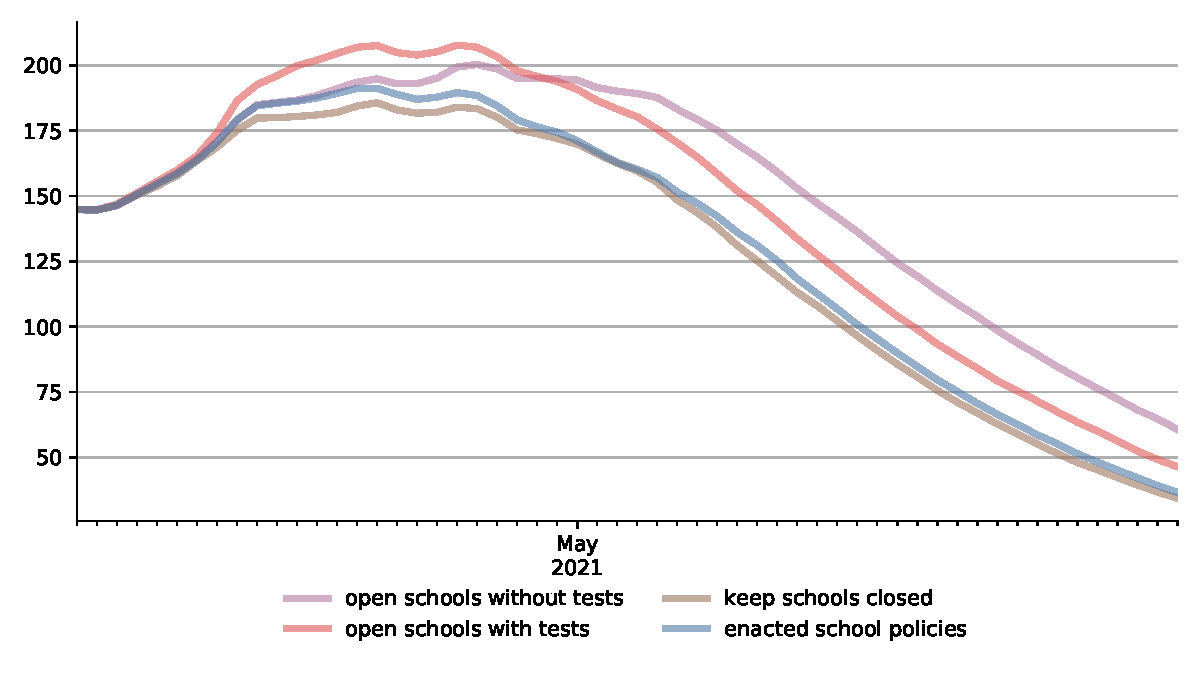
\includegraphics[width=0.9 \textwidth]{../figures/results/figures/scenario_comparisons/school_scenarios/full_new_known_case}
  \end{subfigure}%
  \begin{subfigure}{.6\textwidth}
    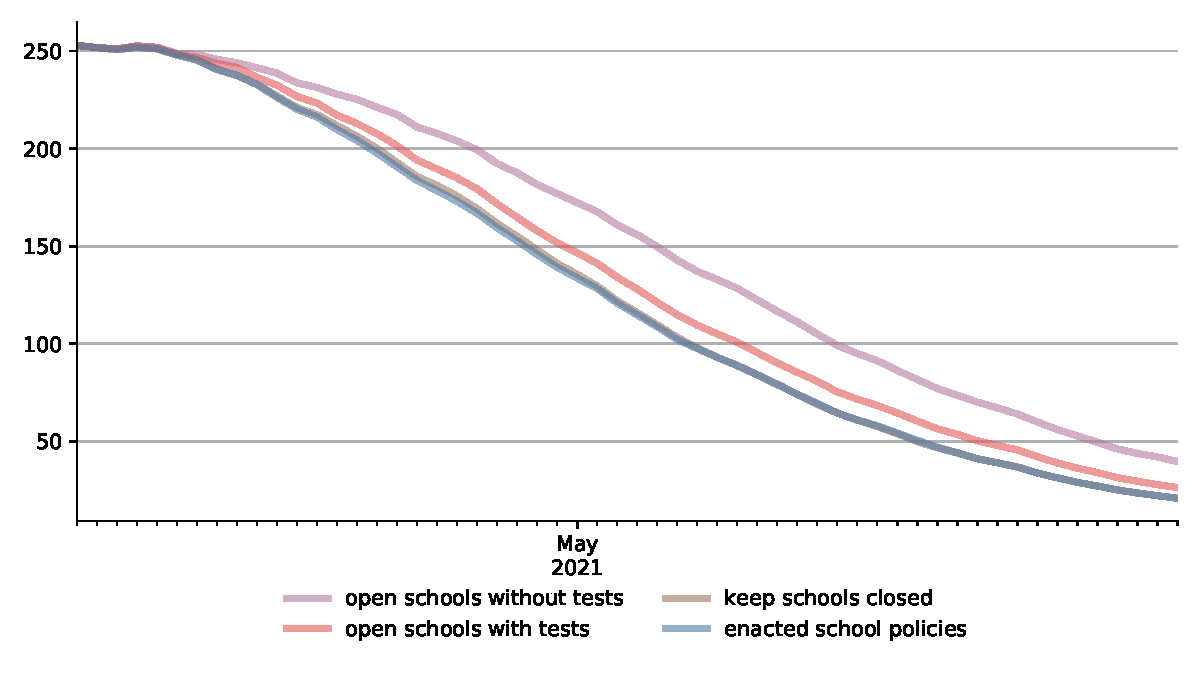
\includegraphics[width=0.9 \textwidth]{../figures/results/figures/scenario_comparisons/school_scenarios/full_newly_infected}
  \end{subfigure}
  \caption{The Effect of Different School Scenarios on Observed and Unobserved Cases}
  \label{fig:school_scenarios_detailed}
\end{figure}


\FloatBarrier

\begin{tabular}{lr}
\toprule
{} &  predicted total infections among 5-14 year olds from Easter until 2021-05-31 \\
scenario                               &                                                                               \\
\midrule
 educ open after easter  without tests &                                             775324 \\
 educ open after easter  with tests    &                                             604078 \\
 close educ after easter               &                                             469274 \\
 baseline                              &                                             478080 \\
\bottomrule
\end{tabular}


\FloatBarrier


\subsection{Shapley Value} % (fold)
\label{sub:shapley_value}

We decompose the effects of different NPIs and seasonality on the infection rates with
Shapley values. Shapley values \citep{Shapley2016} are a concept in game theory to
divide payoffs between a coalition of players. It allows to assign a single value to the
contribution of an NPI or seasonality which takes into account substitutional and
complementary effects with other factors.

More formally, define a coalitional game with $N$ players and a super-additive function
$\nu$ which maps subsets of $N$ to the real numbers. The function $\nu$ is also called
the characteristic function and assigns a value to a coalition. Then, the Shapley value
$\phi$ for player $i$ is

\begin{align*}
    \phi_i(\nu) = \frac{1}{|N| !} \sum_{S \subseteq N \setminus \{i\}} |S| ! (|N| - |S| - 1)! (\nu(S \cup \{i\}) - \nu(S))
\end{align*}

The last term $(\nu(S \cup \{i\}) - \nu(S))$ is the marginal contribution of player $i$
minus the coalition without player $i$. Then, compute the sum of marginal contributions
over all subsets $S$ of $N$ which do not include player $i$. Each marginal contribution
has to be multiplied by all combinations of other players in $S$ which precede $i$ and
all possible combinations of remaining players which follow player $i$ in the coalition.
To arrive at the Shapley value for player $i$, divide the sum by the total number of
combinations.

The Shapley value has some properties.

\begin{description}
  \item[Efficiency] The sum of Shapley values is equal to the value of a coalition
  formed by all players.
  \item[Symmetry] The Shapley does not depend on the label of a player but only on its
  position in the characteristic function.
  \item[Linearity] The Shapley value depends linearly on the values from the
  characteristic function $\nu$.
  \item[Dummy Axiom] The Shapley value of a player who contributes nothing to any
  coalition is 0.
\end{description}

To produce Figure~\ref{fig:2021_scenarios_decomposition} and
Figure~\ref{fig:2021_scenarios_decomposition_tests}, we calculate the Shapley values of
each factor in the comparison on the cumulative number of saved infections between the
main scenario and the scenario without any of the factors for every day. Then, we divide
up the saved infections on a particular day according to the Shapley values for the same
day which yields the daily saved infections for each factor.


% subsection shapley_value (end)